\chapter{Breezy Project: a DOTA 2 competition}
\label{chap:dota}

During the first month of my internship I teamed up with my supervisor \href{https://www.linkedin.com/in/dennis-g-wilson/}{\color{blue}{Assoc. Prof. Dennis Wilson}} and my fellow Research Intern \href{https://www.linkedin.com/in/lucashervier/}{\color{blue}{Lucas Hervier}} to participate in an Evolutionary Reinforcement Learning competition held as part of the international Genetic and Evolutionary Computation Conference, known as GECCO 2020, on the DOTA 2 video game.

\section{Context}
In 2018 the video game industry generated sales of more than US\$130 billion, reaching around 2 billion players around the world. Because video games can provide complex tasks necessitating short- and long-term planning in a controlled environment with no risks to humans \cite{Games_AI}, they also provide an excellent test-bed for Artificial Intelligence (AI) systems. Multiple learning agents have been tested on the Arcade Learning Environment based on Atari 2600 games \cite{Atari}, including Reinforcement Learning (RL) techniques like Deep Q Networks \cite{DQN} and Agent57 \cite{agent57}. Other games such as StarCraft, DOTA2, Mario, or Doom, have also been extensively used as machine learning benchmarks.

Since the reward in games is often sparse, making the learning signal weak, gradient-based methods might struggle for the optimization of neural network parameters. Evolutionary Strategies (ES), which estimate the gradient of the objective function without needing an explicit gradient definition, have been used to optimize Deep Convolutional Neural Networks \cite{CMAES_DL}, and the evolution of synaptic weights have been demonstrated to be competitive with deep RL methods\cite{deep_neuroevo}.\\

In this context, \href{https://web.cs.dal.ca/~dota2/?page_id=353}{\color{blue} {Project Breezy}} is a competition created by Robert SMITH and Malcolm HEYWOOD from Dalhousie University to develop a \href{https://store.steampowered.com/app/570/Dota_2/}{\color{blue}{DOTA 2}}-playing bot evolved with evolutionary algorithms, in a 1-versus-1 symmetrical match-up. 

We entered this competition as an opportunity to try and test neuroevolution algorithms on a complex real-time game, and as a step towards the development of a comprehensive benchmark of Evolutionary Reinforcement Learning algorithms.

\section{DOTA 2 as a RL environment}
\subsection{The game}

\subsection{Challenges}
Evolving Neural Networks to play video games is subject to multiple constraints:
\begin{itemize}
    \item Since DOTA 2 is a real-time game, the generated neural networks needs to be fast to evaluate at each step.
    \item Even sped up, evaluating a neural network requires to run a full game in a simulator, hence the number of evaluations is a strong limiting factor.
    \item Due to the size of the game state provided, generated neural networks might be large hence have many weights to optimize, and some genetic algorithms may struggle due to high dimensionality.
\end{itemize}



\section{Our approach}
\subsection{NEAT and CGP}
\subsection{Map-Elites}
\subsection{Reducing the computation cost}

\section{Results}

\begin{figure}[H]
\centering
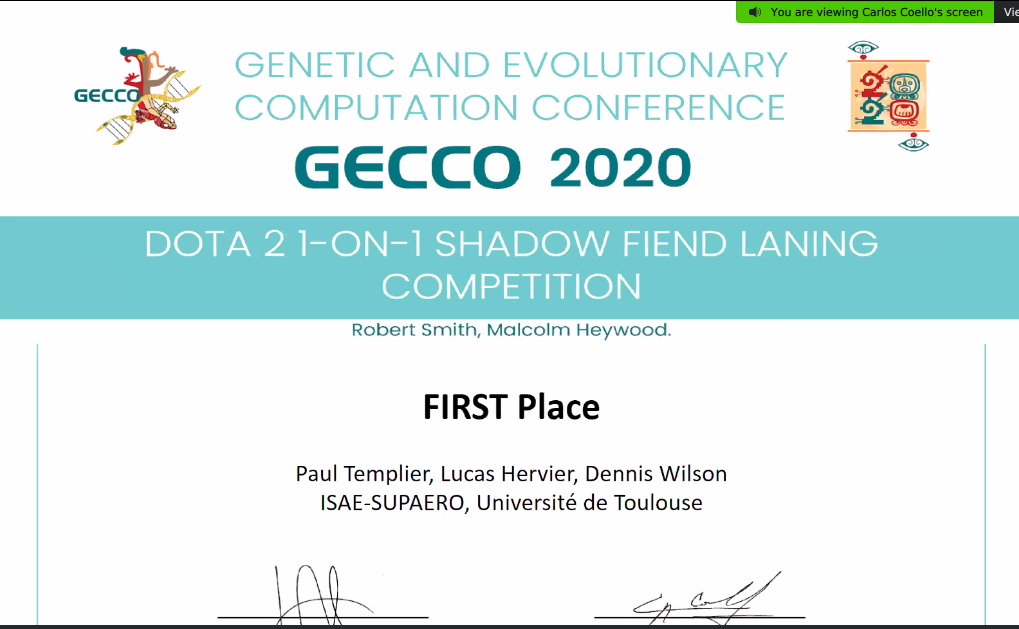
\includegraphics[width=12cm]{images/breezy-win.png}
\caption{Competition results announcement at GECCO 2020}
\end{figure}

%%% Local Variables: 
%%% mode: latex
%%% TeX-master: "isae-report-template"
%%% End: 